\documentclass[10pt]{report}
\usepackage{fullpage}
\usepackage{amsmath}
\usepackage{amsfonts}
\usepackage{amssymb}
\usepackage[version=4]{mhchem}
\usepackage{stmaryrd}
\usepackage{graphicx}
\usepackage{array}
\usepackage{babel}
\usepackage{caption}
\usepackage{color}
\usepackage{float}
\usepackage{parskip}
\usepackage{physics}
\usepackage{subcaption}
\usepackage{caption}
\captionsetup{justification=centering}
\usepackage[export]{adjustbox}
\graphicspath{ {./images/} }

\title{Algoritm de achiziție și compresie în domeniul codului }

\author{Popescu Ervin-Adrian\\444C}
\date{}


\begin{document}
\maketitle

\subsection*{Introducere}

În această lucrare, este propus un algoritm de achiziție a semnalului GNSS bazat pe comprimarea în două etape a domeniului frecvență cod, care împarte offset-ul de frecvență Doppler în mai multe intervale, iar punctele de frecvență multiple sunt comprimate și căutate în fiecare interval în același timp pentru a crește lățimea de bandă de corelare. Această metodă poate depăși limitările căutării convenționale de frecvență Doppler și este potrivită pentru achiziție rapidă în dinamică înaltă.


\subsection*{Sparsificarea semnalului GNSS}
Semnalul de frecvență intermediară (IF) GNSS digital de intrare în jos poate fi exprimat ca

\begin{equation}
    r(n)=A d(n) c(n-\tau) \exp \left[j\left(2 \pi\left(f_{\mathrm{IF}}+f_{\mathrm{d}}\right) n T_{\mathrm{S}}+\varphi\right)\right]+v(n)
    \label{eq:1}
\end{equation}

unde \(A\) este amplitudinea semnalului, \(d\) sunt datele semnalului, \(c\) este codul de împrăștiere, \(f_{\mathrm{IF}}\) este frecvența intermediară, \( f_{\mathrm{d}}\) este decalajul de frecvență Doppler, \(T_{\mathrm{s}}\) este intervalul de eșantionare, \(\tau\) este faza codului, \(v\) este zgomotul și \(\varphi\) este faza purtătoare necunoscută.

Din lucrările anterioare, știm că achiziția semnalului GNSS este posibilă la o rată de eșantionare scăzută prin utilizarea teoriei CS pentru a comprima datele brute ale semnalului GNSS folosind o matrice de măsurare, care poate fi exprimată ca

\begin{equation}
    \mathbf{y}=\boldsymbol{\Phi} \cdot \mathbf{x}
\end{equation}

unde \(\mathbf{x}\) este semnalul original, \(\mathbf{y}\) este vectorul de măsurare, \(\boldsymbol{\Phi} \in R^{M \times N}\) este matricea de măsurare, \(N\) este lungimea semnalului, \(M\) este lungimea de măsurare și \(M<<N\).

Premisa CS este că semnalul este rar. Cu toate acestea, majoritatea semnalelor reale nu sunt rare, dar pot fi exprimate ca

\begin{equation}
    \mathbf{x}=\boldsymbol{\Psi} \cdot \mathbf{a}
\end{equation}

unde \(\Psi\) se numește baza rară a semnalului, \(\mathbf{a}\) este un vector rar.

Deplasarea vectorului de cod de împrăștiere \(\mathbf{c}=[c(0), c(1), \cdots, c(N K-1)] \in R^{N K \times 1}\) pentru a obține matrice de cod \(\mathbf{C}\)

\begin{equation}
    \mathbf{C}=\left[\mathbf{c}_{0}, \mathbf{c}_{1}, \cdots, \mathbf{c}_{N-1}\right]=\left[ \begin{matrix}{cccc}
            c(0)       & c(1)         & \cdots & c(2 K-1)     \\
            c(K)       & c(K+1)       & \cdots & c(3 K-1)     \\
            \vdots     & \vdots       & \ddots & \vdots       \\
            c[(N-1) K] & c[(N-1) K+1] & \cdots & c[(N+1) K-1]
        \end{matrix}\right]
\end{equation}

unde \(N\) este numărul de puncte din \(\mathrm{FFT}\) și \(N=2 \mathrm{~K}\).

Adăugarea zerourilor până la sfârșitul semnalului de intrare \(r(n)\) pentru a-i crește lungimea la \(2 K\), ceea ce poate rezolva problema neperiodicității după procesarea în bloc a codului de răspândire și poate reduce eficient calculul. Poate fi descris ca

\begin{equation}
    \mathbf{r}=\left[r(0), r(1), \cdots, r(K-1), 0_{1 \times K}\right]^{\mathrm{T}}
\end{equation}

Apoi, corelând vectorul de semnal captusit \(\mathbf{r}\) cu matricea codului local de răspândire \(\mathbf{C}\), putem obține vectorul de corelație \(\mathbf{X}\)

\begin{equation}
    \mathbf{X}=\mathbf{C} \cdot \mathbf{r}
\end{equation}

Funcția de corelație (CF) a semnalului de intrare și a codului de răspândire poate fi descrisă ca

\begin{equation}
    X_{i}=<\mathbf{c}_{n}, \mathbf{r}>=\sum_{i=0}^{2 K-1} c(i+n) r(i)=\left \{\begin{matrix}{cc}
        v+2AK\left(1-\frac{|\tau|}{T_{\mathrm{c}}}\right), & |\tau| \leq T_{\mathrm{c}} \\
        v, |\tau|>T_{\mathrm{c}}
    \end{matrix}\right.
\end{equation}

unde \(X_{i}\) este \(i\)-lea element al vectorului de corelație \(\mathbf{X}, \mathbf{c}_{n}\) este \(n\)-lea rând a matricei de cod \(\mathbf{C}\), \(<\cdot>\) este operația de convoluție în timp discret, \(T_{\mathrm{C}}\) este timpul cipului, \(2 A K\) este valoarea maximă de vârf.

După cum se arată în Figura 1, rezultatul corelației \(\mathbf{X}\) poate fi considerat rar dacă \(|2 A K|>>|v|\) în ecuația (7).

\begin{center}
    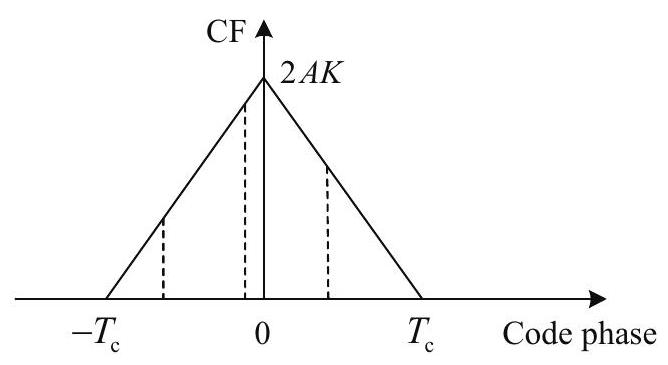
\includegraphics[max width=8cm]{2023_06_04_7690788c3d6419e4c10eg-2}
\end{center}

Figura 1. Modelul de ieșire a corelației.

\subsection*{Achiziție și compresie în domeniul codului}
Conform ecuațiilor (2) și (6), putem folosi matricea de măsurare \(\boldsymbol{\Phi}\) pentru a comprima rezultatul corelației dimensionale \(N \times 1\) \(\mathbf{X}\) pentru a obține datele de măsurare dimensională \(M \times 1\) \(\mathbf{Y}\)


\begin{equation}
    \underset{M \times 1}{\mathbf{Y}}=\underset{M \times N}{\mathbf{\Phi}} \cdot \underset{N \times 1}{\mathbf{X}}= \underset{M \times N}{\mathbf{\Phi}} \cdot \underset{N \times 2 K}{\mathbf{C}} \cdot \underset{2 K \times 1}{\mathbf{r}}
\end{equation}

Matricea de măsurare \(\boldsymbol{\Phi}\) va fi utilă pentru reconstrucția semnalului  atunci când criteriile de proprietate restricționată de izometrie (RIP) sunt îndeplinite. Cu alte cuvinte, fiecare coloană este un vector unitar, iar suma pătratelor tuturor coloanelor îndeplinește limita Welch


\begin{equation}
    \sum_{i=1}^{N} \sum_{j=1}^{N}\left|\left\langle\phi_{i}, \phi_{j}\right\rangle\right|^{2 } \geq \frac{N^{2}}{M}
\end{equation}

Motorul de căutare paralel bazat pe FFT este adoptat pentru a obține vârful de corelație, care convertește operația de convoluție în domeniul timpului în multiplicare în domeniul frecvenței. FFT pentru \(\boldsymbol{\Phi} \cdot\) C sunt luate și înmulțite cu FFT ale \(\mathbf{r}\), apoi luate FFT inversă (IFFT) pentru a obține Y.

Rezultatul corelației \(\mathbf{X}\) poate fi reconstruit din \(\mathbf{Y}\) prin niște algoritmi de reconstrucție, care pot fi descriși după cum urmează


\begin{equation}
    \min \|\mathbf{X}\|_{0} \quad \text { s.t. } \quad \mathbf{Y}=\mathbf{\Phi} \cdot \mathbf{X}
\end{equation}


unde \(\|\cdot\|_{0}\) înseamnă norma \(l_{0}\) care numără numărul de elemente diferite de zero.

Norma \(l_{0}\) este o problemă NP-hard, care poate fi convertită în normă \(l_{2}\) dacă matricea de măsurare \(\boldsymbol{\Phi}\) îndeplinește condiția RIP.


\begin{equation}
    \min \|\mathbf{X}\|_{2}^{2} \quad \text { s.t. } \quad \mathbf{Y}=\boldsymbol{\Phi} \cdot \mathbf{X}
\end{equation}


unde \(\|\cdot\|_{2}\) este norma \(l_{2}\), cunoscută și sub denumirea de norma euclidiană, care este folosită ca mărime standard pentru măsurarea unei diferențe vectoriale.

Metoda celor mai mici pătrate (LSM) este utilizată pentru a reconstrui elementele din datele de măsurare \(\mathbf{Y}[27]\).


\begin{equation}
    \mathbf{X}=\boldsymbol{\Phi}^{\mathrm{T}}\left(\boldsymbol{\Phi} \boldsymbol{\Phi}^{\mathrm{T}}\right)^{-1 } \mathbf{Y}
\end{equation}


Faza corectă a codului și decalajul de frecvență Doppler sunt determinate prin compararea primelor elemente \(K\) din rezultatul corelației \(X\). Înlocuirea corelației circulare cu o reconstrucție comprimată în această metodă scade numărul de corelatori de la \(N+1\) la \(M+1[28]\)

După cum știm, funcția de corelare \(R\left(\tau, f_{\mathrm{d}}\right)\) a codului de împrăștiere poate fi descrisă după cum urmează


\begin{equation}
    R\left(\tau, f_{\mathrm{d}}\right)=2 A K\left(1-\frac{|\tau|}{T_{\mathrm{c}}}\right) \frac{ \sin \left[\pi\left(f_{\mathrm{d}}-f_{i}\right) 2 K T_{\mathrm{s}}\right]}{\sin \left[\pi\left (f_{\mathrm{d}}-f_{i}\right) T_{\mathrm{s}}\right]} \exp [j \gamma(\varphi)]
\end{equation}


unde \(\gamma(\varphi)=\pi\left(f_{\mathrm{d}}-f_{i}\right)(2 K-1) T_{\mathrm{s}}+\varphi, f_ {i}\) este ipoteza frecvenței Doppler.

Putem găsi că \(R\left(\tau, f_{\mathrm{d}}\right)\) este afectat de frecvența Doppler ca o funcție \(\operatorname{sinc}(\cdot)\) și zero al lobului său principal este situat la


\begin{equation}
    f_{\mathrm{d}}=\frac{ \pm 1}{K T_{\mathrm{s}}}+f_{i}
\end{equation}


Lățimea de bandă de corelație \(B_{\mathrm{C}}\) denotă


\begin{equation}
    B_{\mathrm{C}}=\frac{2}{K T_{\mathrm{s}}}
\end{equation}


Prin urmare, intervalul de offset al frecvenței Doppler în fiecare căutare este obținut ca


\begin{equation}
    f_{\mathrm{d}} \in\left[\frac{-1}{K T_{\mathrm{s}}}+f_{i}, \frac{1}{K T_{\mathrm{s} }}+f_{i}\right]
\end{equation}


unde precizia căutării este \(1 /\left(K T_{\mathrm{s}}\right)\).

În algoritmul de mai sus, achiziția este în serie în domeniul frecvenței și va dura mult timp pentru a obține frecvența Doppler în dinamică înaltă.

\section{Achiziție și compresie în două etape cu frecvența codului}
În această secțiune, introducem o nouă compresie în domeniul frecvenței pentru a preprocesa semnalul de intrare pentru a reduce influența offset-ului mare de frecvență Doppler.

\subsection*{Preprocesare de comprimare a domeniului de frecvență}
Semnalul de intrare este înmulțit cu \(\exp \left[j 2 \pi\left(f_{\mathrm{o}}^{i}+f_{\mathrm{c}}^{l}\right)\right) ]\) pentru a produce semnalul mapat \(r_{l}^{\prime}(n)\)


\begin{equation}
    r_{l}^{\prime}(n)=r(n) \exp \left[j 2 \pi\left(f_{\mathrm{o}}^{i}+f_{\mathrm{c}} ^{l}\right) n T_{\mathrm{s}}\right]
\end{equation}


unde \(f_{\mathrm{c}}^{l}\) este intervalele multiple de frecvență purtătoare, \(l \in\{0,1,2, \ldots, L-1\}, L\) este raportul de compresie în frecvență (FCR), pasul de căutare a frecvenței \(f_{\text {pas }}=f_{\mathrm{c}}^{l+1}-f_{\mathrm{c}^{l}} ^{l} f_{\mathrm{o}}^{i}\) este frecvența de pornire în căutarea cu compresie o dată în frecvență, \(i \in\{0,1,2, \ldots, I-1\}, I\) este numărul de sub-purtători, pașii de compresie a frecvenței \(f_{\mathrm{o}}^{i+1}-f_{\mathrm{o}}^{i}=L \cdot f_ {\text {pas }}\).

Prin urmare, offset-ul de frecvență Doppler poate fi exprimat ca

\begin{equation}
    f_{\mathrm{d}}=I \cdot L \cdot f_{\text {pas }}
\end{equation}

Figura 2 prezintă procesul tehnicii de căutare a frecvenței purtătoarei bazată pe cartografiere și suprapunere. Împărțim offset-ul de frecvență Doppler \(f_{\mathrm{d}}\) în compartimente de frecvență sub-purtătoare \(I\) și căutăm puncte de subfrecvență \(L\) separate prin \(f_{\text { pasul }}\) simultan.

\begin{figure}[h]
    \begin{center}
        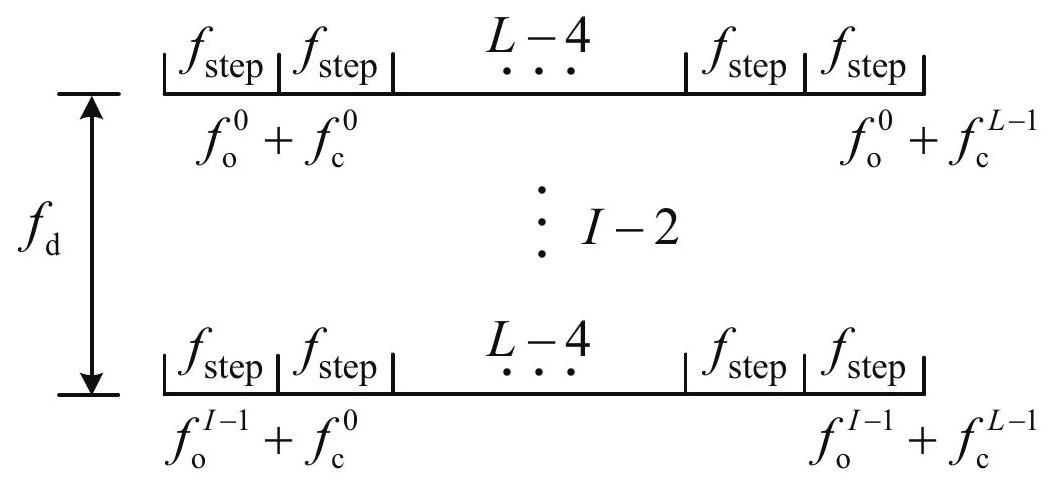
\includegraphics[max width=12cm]{2023_06_04_7690788c3d6419e4c10eg-4}
        \caption*{Figura 2. Diagrama schematică a procesării compresiei în domeniul frecvenței.}
    \end{center}
\end{figure}

Din ecuația (13), putem vedea că dacă frecvența Doppler este mai mare decât lățimea de bandă de corelație \(B_{\mathrm{c}}=2 /\left(K T_{\mathrm{s}}\right)\), valoarea corelației este atenuată serios. În consecință, pasul de căutare a frecvenței ar trebui să satisfacă \(f_{\text {pas }} \leq B_{\mathrm{c}} / 2\), asigurându-se că cel puțin două puncte de frecvență de achiziție învecinate sunt situate în lățimea de bandă de corelare \( B_{\mathrm{c}}\), care este benefic pentru îmbunătățirea performanței achiziției, așa cum se arată în Figura 3a. Totuși, dacă \(f_{\text {pas }}>B_{\mathrm{c}}\), frecvența de achiziție a vecinului depășește lățimea de bandă de corelație \(B_{\mathrm{c}}\), determinând valoarea corelației scăderea și eșecul achiziției, așa cum este ilustrat în figura \(3 \mathrm{~b}\).

Apoi, semnalele mapate care corespund aceleiași faze de cod sunt suprapuse împreună. În consecință, obținem semnalul de intrare preprocesat


\begin{equation}
    r_{l}^{\prime \prime}(n)=\sum_{l=0}^{L-1} r_{l}^{\prime}(n)
\end{equation}

Lățimea de bandă de corelație a achiziției de compresie este îmbunătățită prin preprocesarea în domeniul frecvenței, care poate fi exprimată ca


\begin{equation}
    B_{\mathrm{c}}^{\prime}=(L-1) f_{\text {pas }}+B_{\mathrm{c}}
\end{equation}


În comparație cu metoda tradițională de căutare a frecvenței Doppler, binurile de frecvență \(L\) sunt căutate simultan în această metodă, ceea ce poate reduce numărul de căutare și timpul de achiziție.

\begin{figure}[h]
    \centering
    \begin{subfigure}[b]{0.4\textwidth}
        \centering
        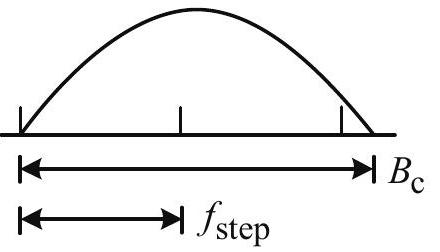
\includegraphics[width=0.5\textwidth]{2023_06_04_7690788c3d6419e4c10eg-5(1).jpg}
        \caption{}
    \end{subfigure}
    \begin{subfigure}[b]{0.4\textwidth}
        \centering
        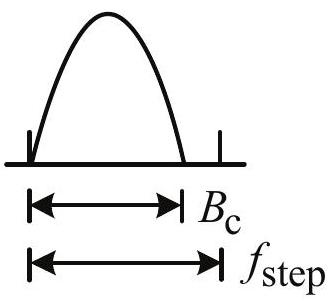
\includegraphics[width=0.4\textwidth]{2023_06_04_7690788c3d6419e4c10eg-5.jpg}
        \caption{}
    \end{subfigure}
    \caption*{Figura 3. Relația dintre pasul de căutare a frecvenței și lățimea de bandă de corelație: (a) \(f_{\text {pas }} \leq B_{\mathrm{c}} / 2\); (b) \(f_{\text {pas }}>B_{\mathrm{c}}\).
    }
\end{figure}

\subsection*{Procesul algoritmului}
Procesele detaliate și simple ale algoritmului de achiziție GNSS propus sunt prezentate în Algoritmul 1 și Figura 4.

\begin{figure}[h]
    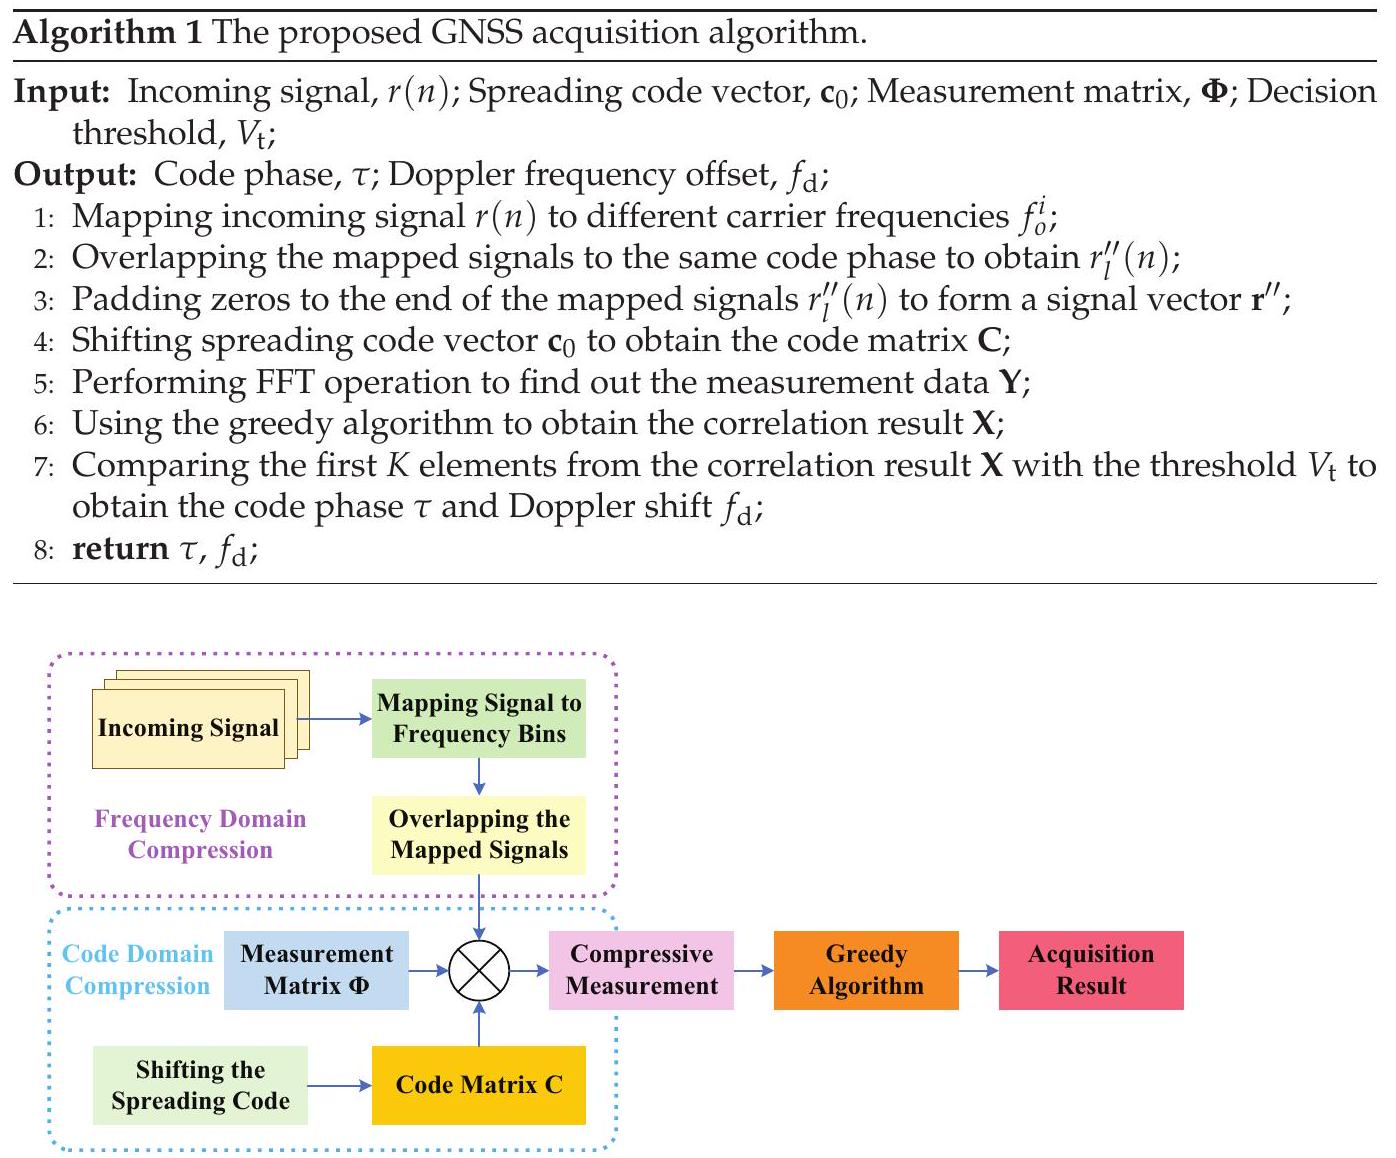
\includegraphics[max width=15cm, center]{2023_06_04_7690788c3d6419e4c10eg-5(2)}
    \caption*{Figura 4. Achiziția semnalului GNSS bazată pe compresia frecvenței codului.}
\end{figure}

\subsection*{Analiza probabilității de detecție}
Presupunând că o matrice Hadamard parțială este adoptată ca matrice de măsurare pentru a evalua performanța algoritmului propus, următoarele două ipoteze determină statistica de test pentru detectarea semnalului

\begin{equation}
    \tilde{\mathbf{y}}=\left\{\begin{array}{cc}
        \boldsymbol{\Phi}_{1} \mathbf{w} și H_{0} \\
        \boldsymbol{\Phi}_{1}(\mathbf{x}+\mathbf{w}) și H_{1}
    \end{array}\right.
\end{equation}


unde \(\boldsymbol{\Phi}_{1} \in \mathbf{R}^{\left(M T_{\mathrm{p}} / \alpha_{c}\right) \times N}\) denotă o matrice Hadamard parțială aleatorie, \(\alpha_{c}\) este factorul maxim de sub-eșantionare, \(T_{\mathrm{p}}\) este perioada spectrului de extindere, \(H_{1}\) denotă semnalul este prezent și aliniat corect cu replica locală, \(H_{0}\) indică faptul că semnalul este absent sau nu este aliniat corect cu replica locală.

În consecință, funcția de densitate de probabilitate a \(\tilde{\mathbf{y}}\) în ipoteza \(H_{1}\) este prezentată după cum urmează:


\begin{equation}
    p\left(\widetilde{\mathbf{y}} \mid \widehat{\overline{\mathbf{x}}}, H_{1}\right)=\frac{1}{(2 \pi)^{ \left(M / \alpha_{\mathrm{c}}\right) / 2}\left|\sigma^{2} \boldsymbol{\Phi}_{1} \boldsymbol{\Phi}_{1}^ {\mathrm{T}}\right|^{1 / 2}} \exp \left[-\frac{1}{2}(\mathbf{W})^{\mathrm{T}}\left(\sigma^{2} \boldsymbol{\Phi}_{1} \boldsymbol{\Phi}_{1}^{\mathrm{T}}\right)^{-1}(\mathbf{W})\right ]
\end{equation}


unde \(\mathbf{W}=\widetilde{\mathbf{y}}-\mathbf{D} \widehat{\mathbf{x}}, \mathbf{D}=\boldsymbol{\Phi}_{1} \cdot \Psi\) și \(\widehat{\mathbf{x}}\) indică


\begin{equation}
    \widehat{\mathbf{x}}=\left(\boldsymbol{\Phi}_{1} \boldsymbol{\Phi}_{1}^{\mathrm{T}}\right)^{-1} \ boldsymbol{\Phi}_{1}^{\mathrm{T}} \tilde{\mathbf{y}}
\end{equation}


\(\widehat{\overline{\mathbf{x}}}\) denotă estimarea cu probabilitatea maximă (MLE) a \(\mathbf{x}\) sub \(H_{1}\), care este prezentată ca


\begin{equation}
    \widehat{\overline{\mathbf{x}}}=\left(\mathbf{D}^{\mathrm{T}}\left(\sigma^{2} \boldsymbol{\Phi}_{1} \ boldsymbol{\Phi}_{1}^{\mathrm{T}}\right)^{-1} \mathbf{D}\right)^{-1} \mathbf{D}^{\mathrm{T} }\left(\sigma^{2} \boldsymbol{\Phi}_{1} \boldsymbol{\Phi}_{1}^{\mathrm{T}}\right)^{-1} \tilde{\ mathbf{y}}
\end{equation}


Dacă pragul \(\eta\) este selectat pentru a atinge probabilitatea de alarmă falsă necesară, performanța de detecție poate fi obținută ca


\begin{equation}
    P_{d}=\operatorname{Pr}\left(\Gamma_{\tilde{\mathbf{y}}}>\eta \mid H_{1}\right)=Q_{\bar{\chi}_{M T_{p} / \alpha_{c}}^{2 \lambda}(\lambda)}(\eta)
\end{equation}


unde \(\Gamma_{\tilde{y}}\) este o distribuție chi-pătrat noncentrală cu \(M T_{\mathrm{p}} / \alpha_{c}\) grade de libertate, care este exprimată ca


\begin{equation}
    \Gamma_{\tilde{\mathbf{y}}}=\tilde{\mathbf{y}}^{\mathrm{T}}\left(\sigma^{2} \boldsymbol{\Phi}_{1} \boldsymbol{\Phi}_{1}^{\mathrm{T}}\right)^{-1} \mathbf{D}\left(\mathbf{D}^{\mathrm{T}}\left( \sigma^{2} \boldsymbol{\Phi}_{1} \boldsymbol{\Phi}_{1}^{\mathrm{T}}\right)^{-1} \mathbf{D}\right) ^{-1} \mathbf{D}^{\mathrm{T}}\left(\sigma^{2} \boldsymbol{\Phi}_{1} \boldsymbol{\Phi}_{1}^{\ mathrm{T}}\right)^{-1} \tilde{\mathbf{y}}
\end{equation}


unde \(\lambda\) este un parametru non-centralitate specificat de

\begin{equation}
    \lambda=\sigma^{-2}\left(\mathbf{x}^{\mathrm{T}}\right)^{-1} \boldsymbol{\Phi}_{1}^{\mathrm{T }}\left(\mathbf{\Phi}_{1} \mathbf{\Phi}_{1}^{\mathrm{T}}\right)^{-1} \mathbf{\Phi}_{1 } \mathbf{x}
\end{equation}


\subsection*{Analiza complexității}
Complexitatea algoritmului propus constă din trei părți: preprocesarea compresiei în domeniul frecvenței, compresia domeniului codului și reconstrucția semnalului, dintre care prima și a treia sunt părțile principale, iar a doua parte poate fi ignorată deoarece elementele matricei de măsurare sunt -1 sau 1. În această lucrare, am ales algoritmul Orthogonal Matching Pursuit (OMP) pentru reconstrucția semnalului, a cărui complexitate este \(O\left(N \cdot\left(\log _{2}(N)\right)^{2}\right)\).\@ Tabelul 1 prezintă complexitățile algoritmului de achiziție în serie, algoritmul de achiziție PMF-FFT, algoritmul de achiziție de compresie de cod (CC) și algoritmul de achiziție de compresie de frecvență de cod (CFC) propus.

Tabelul 1. Tabelul complexităților algoritmilor.

\begin{center}
    \begin{tabular}{cc}
        \hline
        Algoritm de achiziție și complexitate                                                                    \\
        \hline
        Algoritm de achiziție în serie  & \(O\left(N^{2} \cdot I \cdot L\right)\)                                \\
        Algoritmul de achiziție PMF-FFT & \(O\left(N \cdot\left(L \cdot \log _{2}(L)+N\right)\right)\)           \\
        Algoritm de achiziție CC        & \(O\left(N \cdot\left(\log _{2}(N)\right)^{2} \cdot I \cdot L\right)\) \\
        Algoritm de achiziție CFC       & \(O\left(N \cdot\left(\log _{2}(N)\right)^{2} \cdot I\right)\)         \\
        \hline
    \end{tabular}
\end{center}
\end{document}